\documentclass[a4paper,12pt]{article} 
\usepackage{geometry}
\usepackage{wrapfig}
\geometry{
	a4paper,
	total={170mm,257mm},
	left=10mm,
	right=10mm,
	top=20mm,
}
\usepackage{titlesec}
\titlelabel{\thetitle.\quad} %точка в section

%%% Работа с русским языком
\usepackage{cmap}                           % поиск в PDF
\usepackage{mathtext} 			 	       % русские буквы в формулах
\usepackage[T2A]{fontenc}               % кодировка
\usepackage[utf8]{inputenc}              % кодировка исходного текста
\usepackage[english,russian]{babel}  % локализация и переносы

%Математика
\usepackage{amsmath,amsfonts,amssymb,amsthm,mathtools} % AMS
\usepackage{icomma} % "Умная" запятая

%% Шрифты
\usepackage{euscript}	 % Шрифт Евклид
\usepackage{mathrsfs} % Красивый матшрифт

\usepackage{gensymb}
\usepackage{graphicx}
\usepackage{setspace}
\usepackage{tabularx}
\usepackage{longtable}
\usepackage{icomma}
\usepackage{euscript}
\usepackage{float}
\usepackage{cutwin}
\usepackage{adjustbox}
\usepackage{dashbox}
\usepackage[normalem]{ulem}	
\usepackage[babel=true]{microtype}
\RequirePackage[T1]{fontenc}
\usepackage{amsmath,amsfonts,amssymb,amsthm,mathrsfs,mathtools} 
\usepackage{xcolor}         
\usepackage{enumitem}     
\usepackage{xpatch}       
\usepackage{cancel}                  
\usepackage{upgreek}                 
\usepackage{lipsum}                  
\usepackage[version=4]{mhchem}       
\usepackage{multirow}                
\usepackage{stackengine}             
\usepackage{tikz}         
\usepackage{hyperref}
\hypersetup{colorlinks=true,urlcolor=blue}       
\usetikzlibrary{positioning}         
\usepackage{titletoc}                 
\usepackage{chngcntr}              
\usepackage{fancyhdr}                
\usepackage{makecell}                
\usepackage{indentfirst}             
\usepackage{tocloft}                 
\usepackage{soul}                   
\usepackage[stable]{footmisc}       
\usepackage{subfig}  
\usepackage{comment}   
\usepackage{physics}               


\mathtoolsset{showonlyrefs=true}


\theoremstyle{definition}
\newtheorem*{definition}{Определение}
\newtheorem{statement}{Предложение}[section]
\newtheorem{lemma}{Лемма}[section]
\newtheorem{theorem}{Теорема}[section]
\newtheorem*{theoremn}{Теорема}
\newtheorem*{corollary}{Следствие}
\newtheorem*{example}{Пример}
\newtheorem*{note}{Замечание}
\newtheorem*{problem}{Задача}


\counterwithout{footnote}{section}\DeclareRobustCommand{\divby}{%
	\mathrel{\text{\vbox{\baselineskip.65ex\lineskiplimit0pt\hbox{.}\hbox{.}\hbox{.}}}}%
}

\newcommand{\dotpr}[2]{\bra{#1}\ket{#2}}
% \let\AA\relax
\let\emptyset\varnothing
\DeclareMathOperator*{\esssup}{ess sup}
\DeclareMathOperator*{\ord}{ord}
\DeclareMathOperator*{\supp}{supp}
\DeclareMathOperator*{\pr}{pr}
\DeclareMathOperator*{\Ker}{Ker}
\DeclareMathOperator*{\Vol}{Vol}
\DeclareMathOperator*{\rg}{rk}
\DeclareMathOperator*{\Ima}{Im}
\DeclareMathOperator*{\Alt}{Alt}
\DeclareMathOperator*{\Sym}{Sym}
\newcommand{\eqdef}{\stackrel{\text{\tiny{def}}}{=}}
\newcommand{\pp}{\partial}
% \newcommand{\AA}{\mathcal{A}}
\newcommand{\BB}{\mathcal{B}}
\newcommand{\MM}{\mathbb{M}}
\newcommand{\NN}{\mathbb{N}}
\newcommand{\ZZ}{\mathbb{Z}}
\newcommand{\QQ}{\mathbb{Q}}
\newcommand{\RR}{\mathbb{R}}
\newcommand{\CC}{\mathbb{C}}
\newcommand{\FFF}{\mathbb{F}}
\newcommand{\DD}{\mathcal{D}}
\newcommand{\FF}{\mathcal{F}}
\newcommand{\sS}{\mathcal{S}}
\newcommand*\circled[1]{\tikz[baseline=(char.base)]{
		\node[shape=circle,draw,inner sep=2pt] (char) {#1};}}

%%% Заголовок
\author{Шерхалов Денис Б02-204и}
\title{Лабораторная работа 4.4.4 \\
	\textbf{Интерферометр Фабри-Перо}}
\date{\today}

\begin{document}
	
{\Large \maketitle}

	\paragraph*{Цель работы:} В данной работе по результатам измерения диаметров интерференционных колец с
  использованием ртутной и натриевой ламп будут определены характеристики
  интерферометра Фабри-Перо: база интерферометра, добротность, линейная дисперсия,
  аппаратная разрешающая способность. Также были определены число интерферирующих лучей,
  разность длин волн для линий пары колец.
	\paragraph*{В работе используются:} ртутная и натриевая лампы, интерферометры Фабри-Перо, катетометры, линзы, светофильтры, оптические скамьи.

\section{Введение}
\begin{figure}[H]
	\begin{minipage}[h]{0.55\linewidth}
		\center{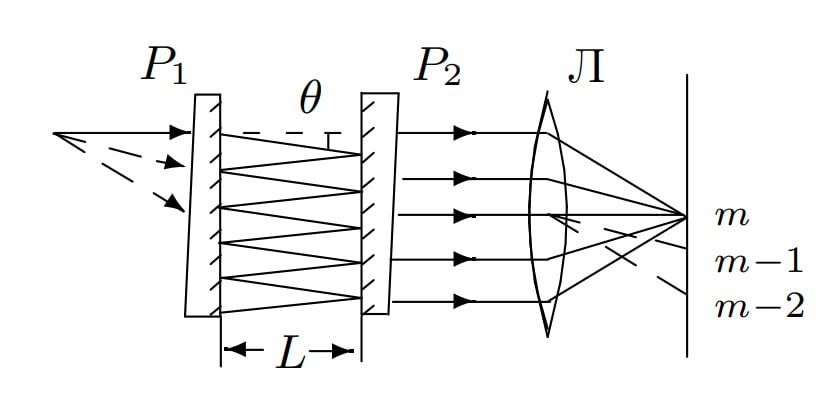
\includegraphics[width=0.95\linewidth]{ifp.png}}
	\end{minipage}
	\begin{minipage}[h]{0.5\linewidth}
		\center{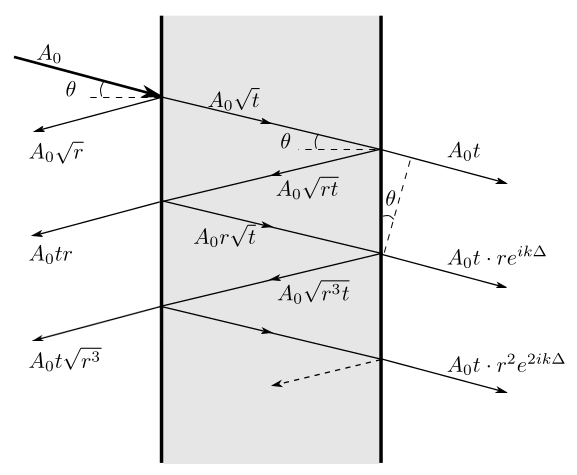
\includegraphics[width=0.95\linewidth]{fp.png}}
	\end{minipage}
  \caption[]{\label{fig:ifp} Интерферометр Фабри-Перо}
\end{figure}

Интерферометр Фабри–Перо состоит из двух стеклянных (или кварцевых) пластин P1 и P2,
внутренние плоские поверхности которых
хорошо отполированы (с точностью до $10^{-2}\lambda$) и установлены параллельно друг
другу. На эти поверхности наносятся хорошо отражающие покрытия. Наружные поверхности
пластин обычно составляют небольшой угол с внутренними, чтобы световой блик,
отраженный от наружных поверхностей, не мешал наблюдениям. Интерферометр Фабри–Перо можно
рассматривать как плоскопараллельную воздушную пластину, на которой происходят
многократные отражения и интерференция световых лучей. Интерференционная картина,
наблюдаемая в фокальной плоскости линзы Л, состоит из концентрических колец равного
наклона. Для двух соседних лучей, распространяющихся между зеркалами интерферометра
под углом $\theta$, разность хода определяется соотношением
\begin{align*}
\Delta = 2L\cos\theta
\end{align*}
где $L$ --- расстояние между зеркалами.
Разрешающей способностью прибора называют величину
\begin{align*}
R = \frac{\lambda}{\delta\lambda}
\end{align*}
разрешающая способность характеризует возможность прибора различать
две близкие спектральные линии с длинами волн $\lambda$ и $\lambda+\delta\lambda$

Угловая дисперсия определяется как
\begin{align*}
D = \frac{d\varphi}{d\lambda}
\end{align*} 
По величине угловой дисперсии можно определить угловое расстояние между двумя
близкими спектральными линиями: $\delta\varphi = D\delta\lambda$

Дисперсионная область – предельная ширина спектрального интервала $\Delta\lambda$ прибора, для которой дифракционные максимумы соседних порядков не перекрываются. Она определяет диапазон
длин волн, при которых прибор может быть использоан для анализа спектра.

В случае интерферометра Фабри-Перо интерференционные
максимумы будут наблюдаться для волн, падающих под углами $\theta_{m}$, удовлетворяющими
условию:
\begin{equation}\label{max_inter}
    2L\cos{\theta_{m}} = m\lambda,
\end{equation}
где $L$ - база интерферометра. Для малых углов выражение можно переписать как 
\begin{equation}
\label{eq:1}
\theta_m^2 = 2 - \frac{\lambda}{L}m
\end{equation}
Так как  $\theta(i) = \frac{d(i)}{2f}$, где $f$ --- фокусное расстояние линзы, стоящей после интерферметра, а $d(i)$ --- диаметр i-ого кольца, можно
получить зависимость угла на максимум интерференции от его номера или диаметра кольца 
\begin{equation}
\label{eq:2}
\frac{d^2(i)}{4f^2} = \theta^2(i) = \text{const} + \frac{i\lambda}{L}
\end{equation}

Выражение можно преобразовать для получения угловой дисперсии:
\begin{equation}
    D_{\text{угл}} \approx -\frac{1}{\lambda \theta_{m}},
\end{equation}
где $\theta_{m} = \frac{d}{2f}$ в данной работе ($f$ -- фокусное расстояние используемой в работе линзы).

Также для малых углов условие возникновения  интерференционного кольца можно записать в виде:
\begin{equation}
    \frac{\lambda}{L} = \frac{1}{4f^2}\frac{\Delta(d^2_i)}{\Delta(i)},
\end{equation}

Отсюда следует используемая в работе формула для линейной дисперсии, которая используется в работе:
\begin{equation}
    D = \frac{2f^{2}}{\lambda d}
\end{equation}

Аппаратная разрешающая способность для порядка спектра $m \approx \frac{2L}{\lambda}$ может быть найдена как:
\begin{equation}
    R = \frac{\lambda}{\delta \lambda} = \frac{\pi \sqrt{r}}{1 - r}m = Nm,
\end{equation}
где $N = \dfrac{\pi \sqrt{r}}{1 - r}$ -- число интерферирующих лучей.

Дисперсионная область интерферометра Фабри-Перо может быть найдена по следующей формуле:
\begin{equation}
    \Delta \lambda = \frac{\lambda^{2}}{2L}.
\end{equation}
\subsection*{Схема установки}
В работе используются ртутная и натриевая лампы; интерферометры Фабри-Перо,
катетометры, линзы, светофильтры, оптические скамьи.
\begin{figure}[htbp]
\centerline{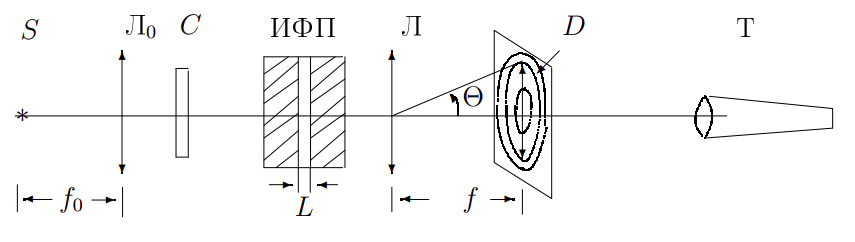
\includegraphics[width=0.7\textwidth]{ust.png}}
\caption[]{\label{fig:scheme} Схема установки}
\end{figure}

На схеме $S$ --- лампа, $ Л_0 $ --- линза, $ C $ --- светофильтр, ИФП --- интерферометр
Фабри-Перо, $T$ --- зрительная труба. Диаметры колец измеряются с помощью микроскопа
катетометра.

\begin{figure}[H]
	\begin{minipage}[h]{0.23\linewidth}
		\center{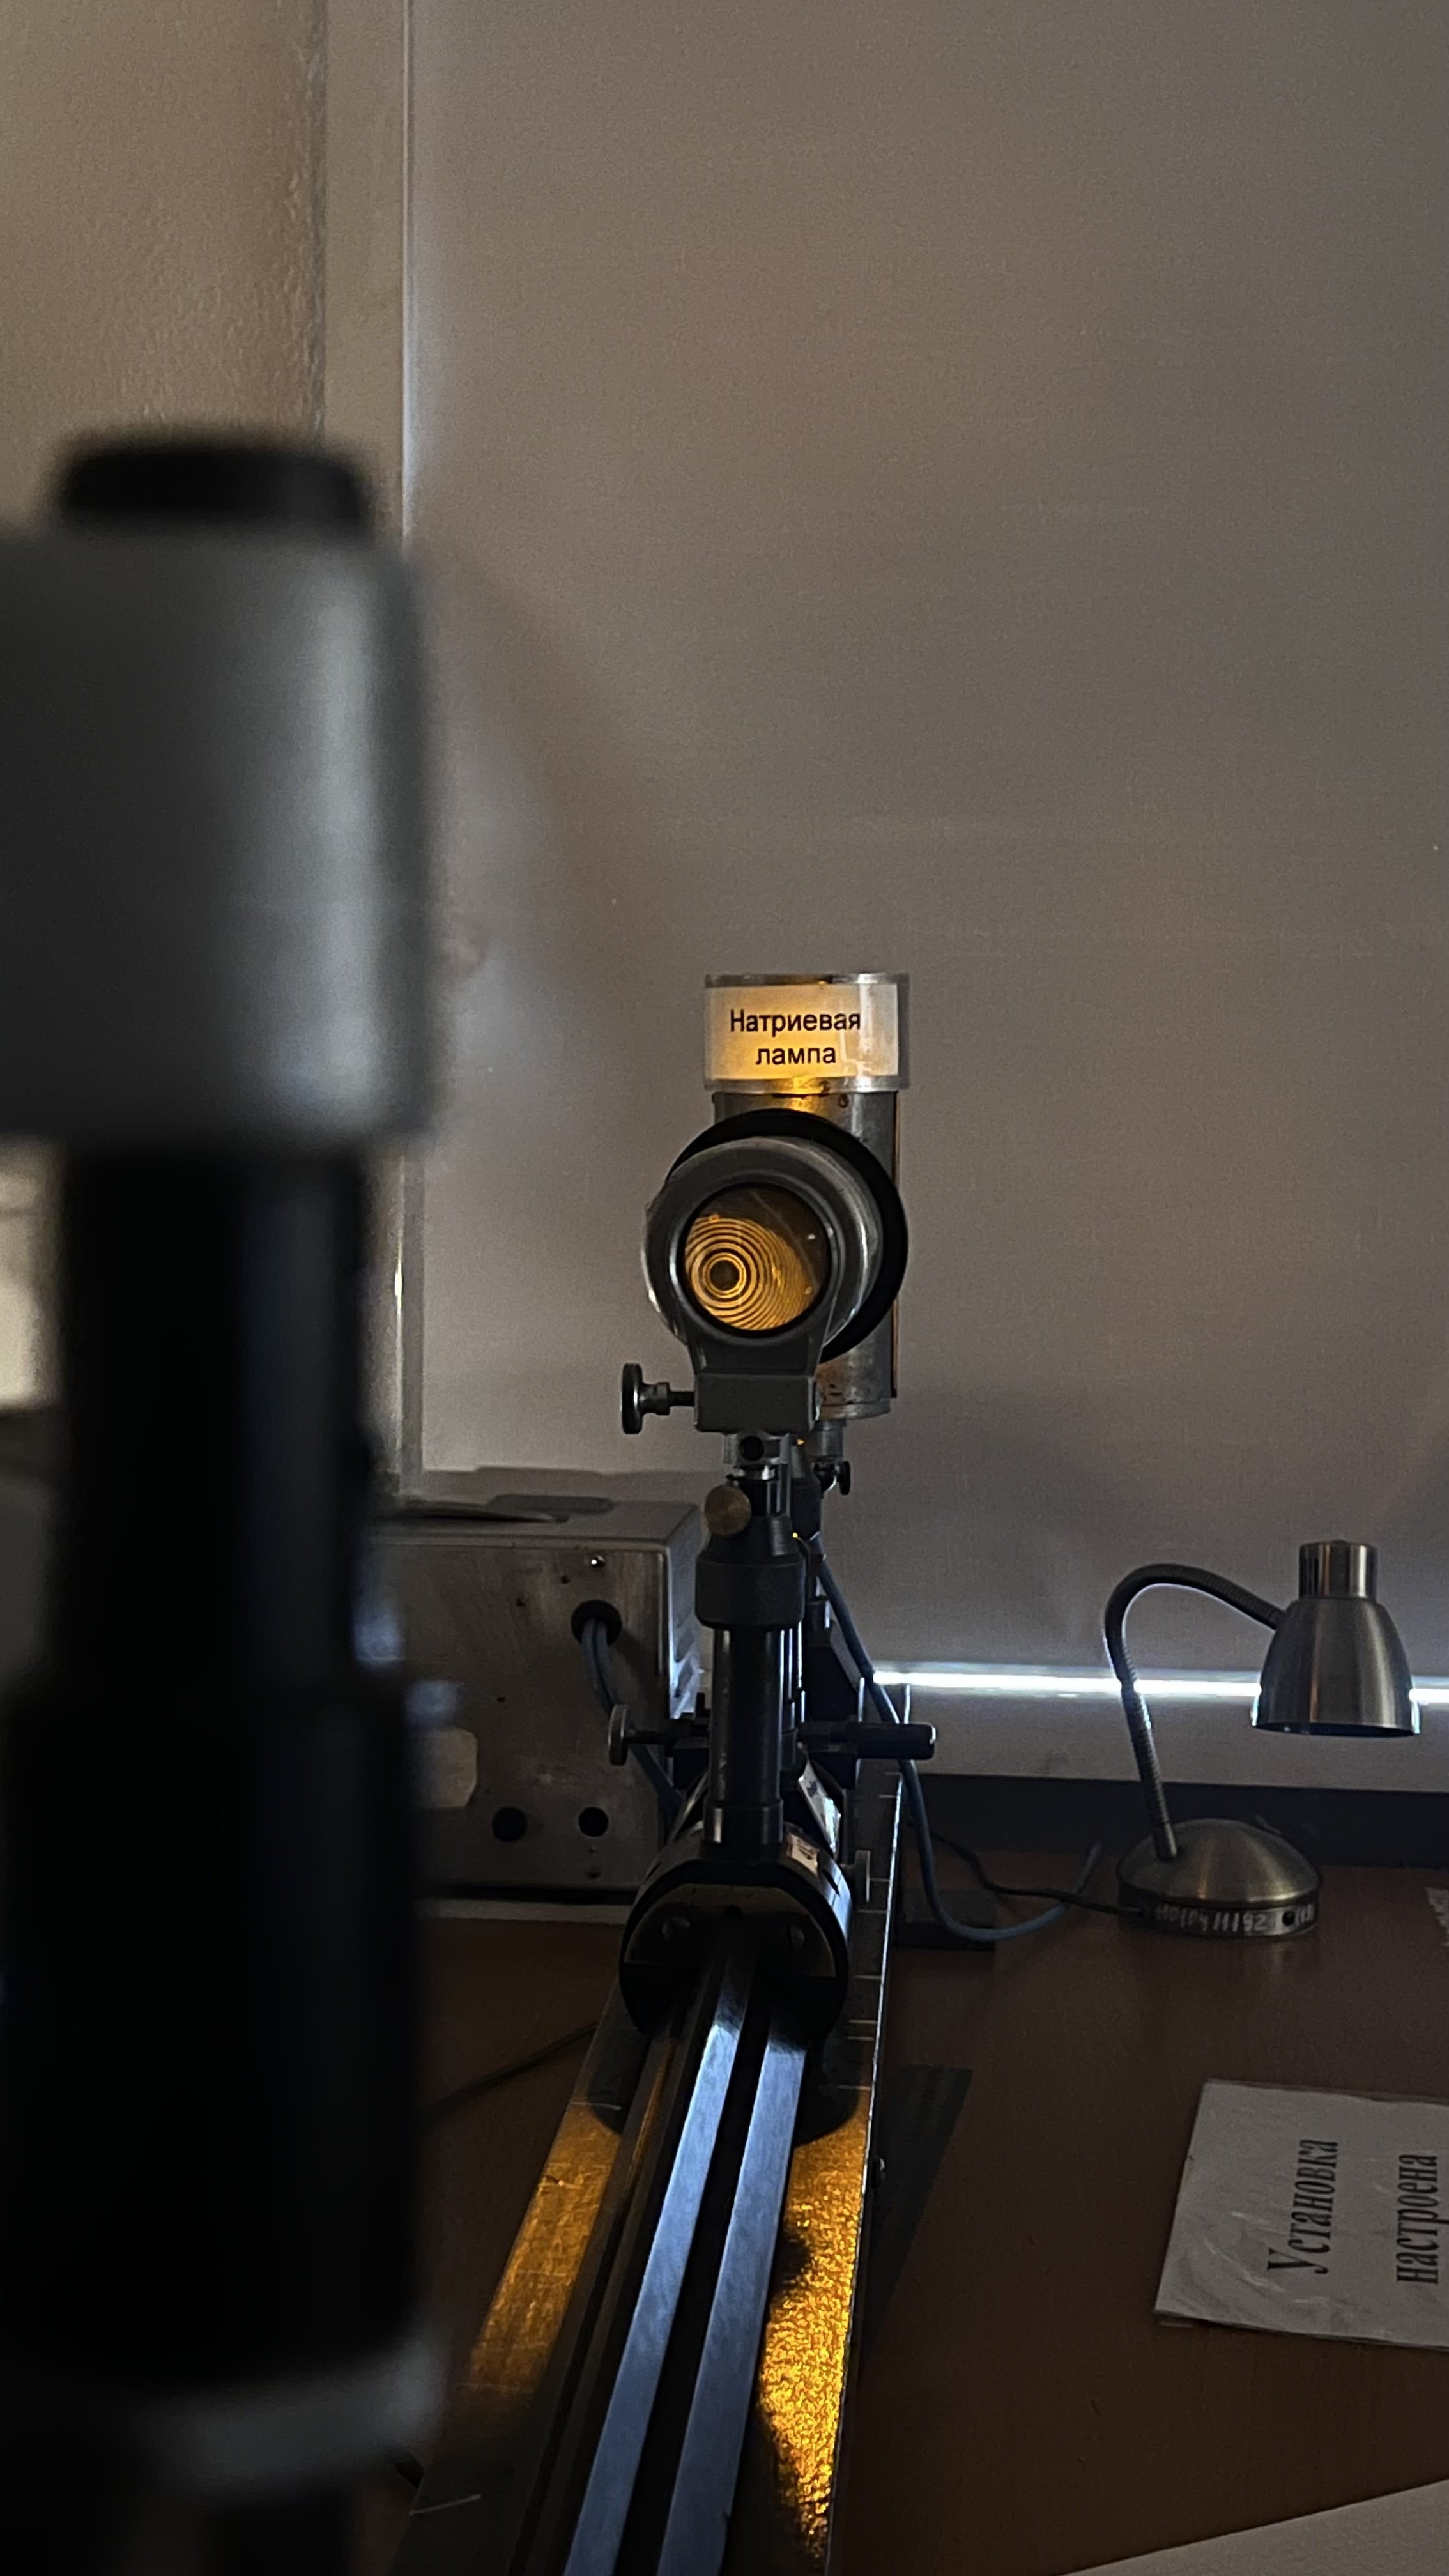
\includegraphics[width=0.95\linewidth]{natriy.png}}
	\end{minipage}
\end{figure}

\section{Выполнение}
\subsection{Характеристики интерферометра Фабри-Перо}
$$R = 0.77 \text{ м} \qquad \qquad L = 146 \text{ м} \qquad \qquad f = 50 \text{ мм}$$
\subsection{Натриевая лампа}
В ходе работы измерены координаты рыжих колец от натриевой лампы. Видно их не менее 24. Измерения координат колец происходило с помощью
микроскопа катетометра с погрешностью $\Delta {R} = 0.02$ мм.

\begin{figure}[H]
	\begin{minipage}[h]{0.5\linewidth}
		\center{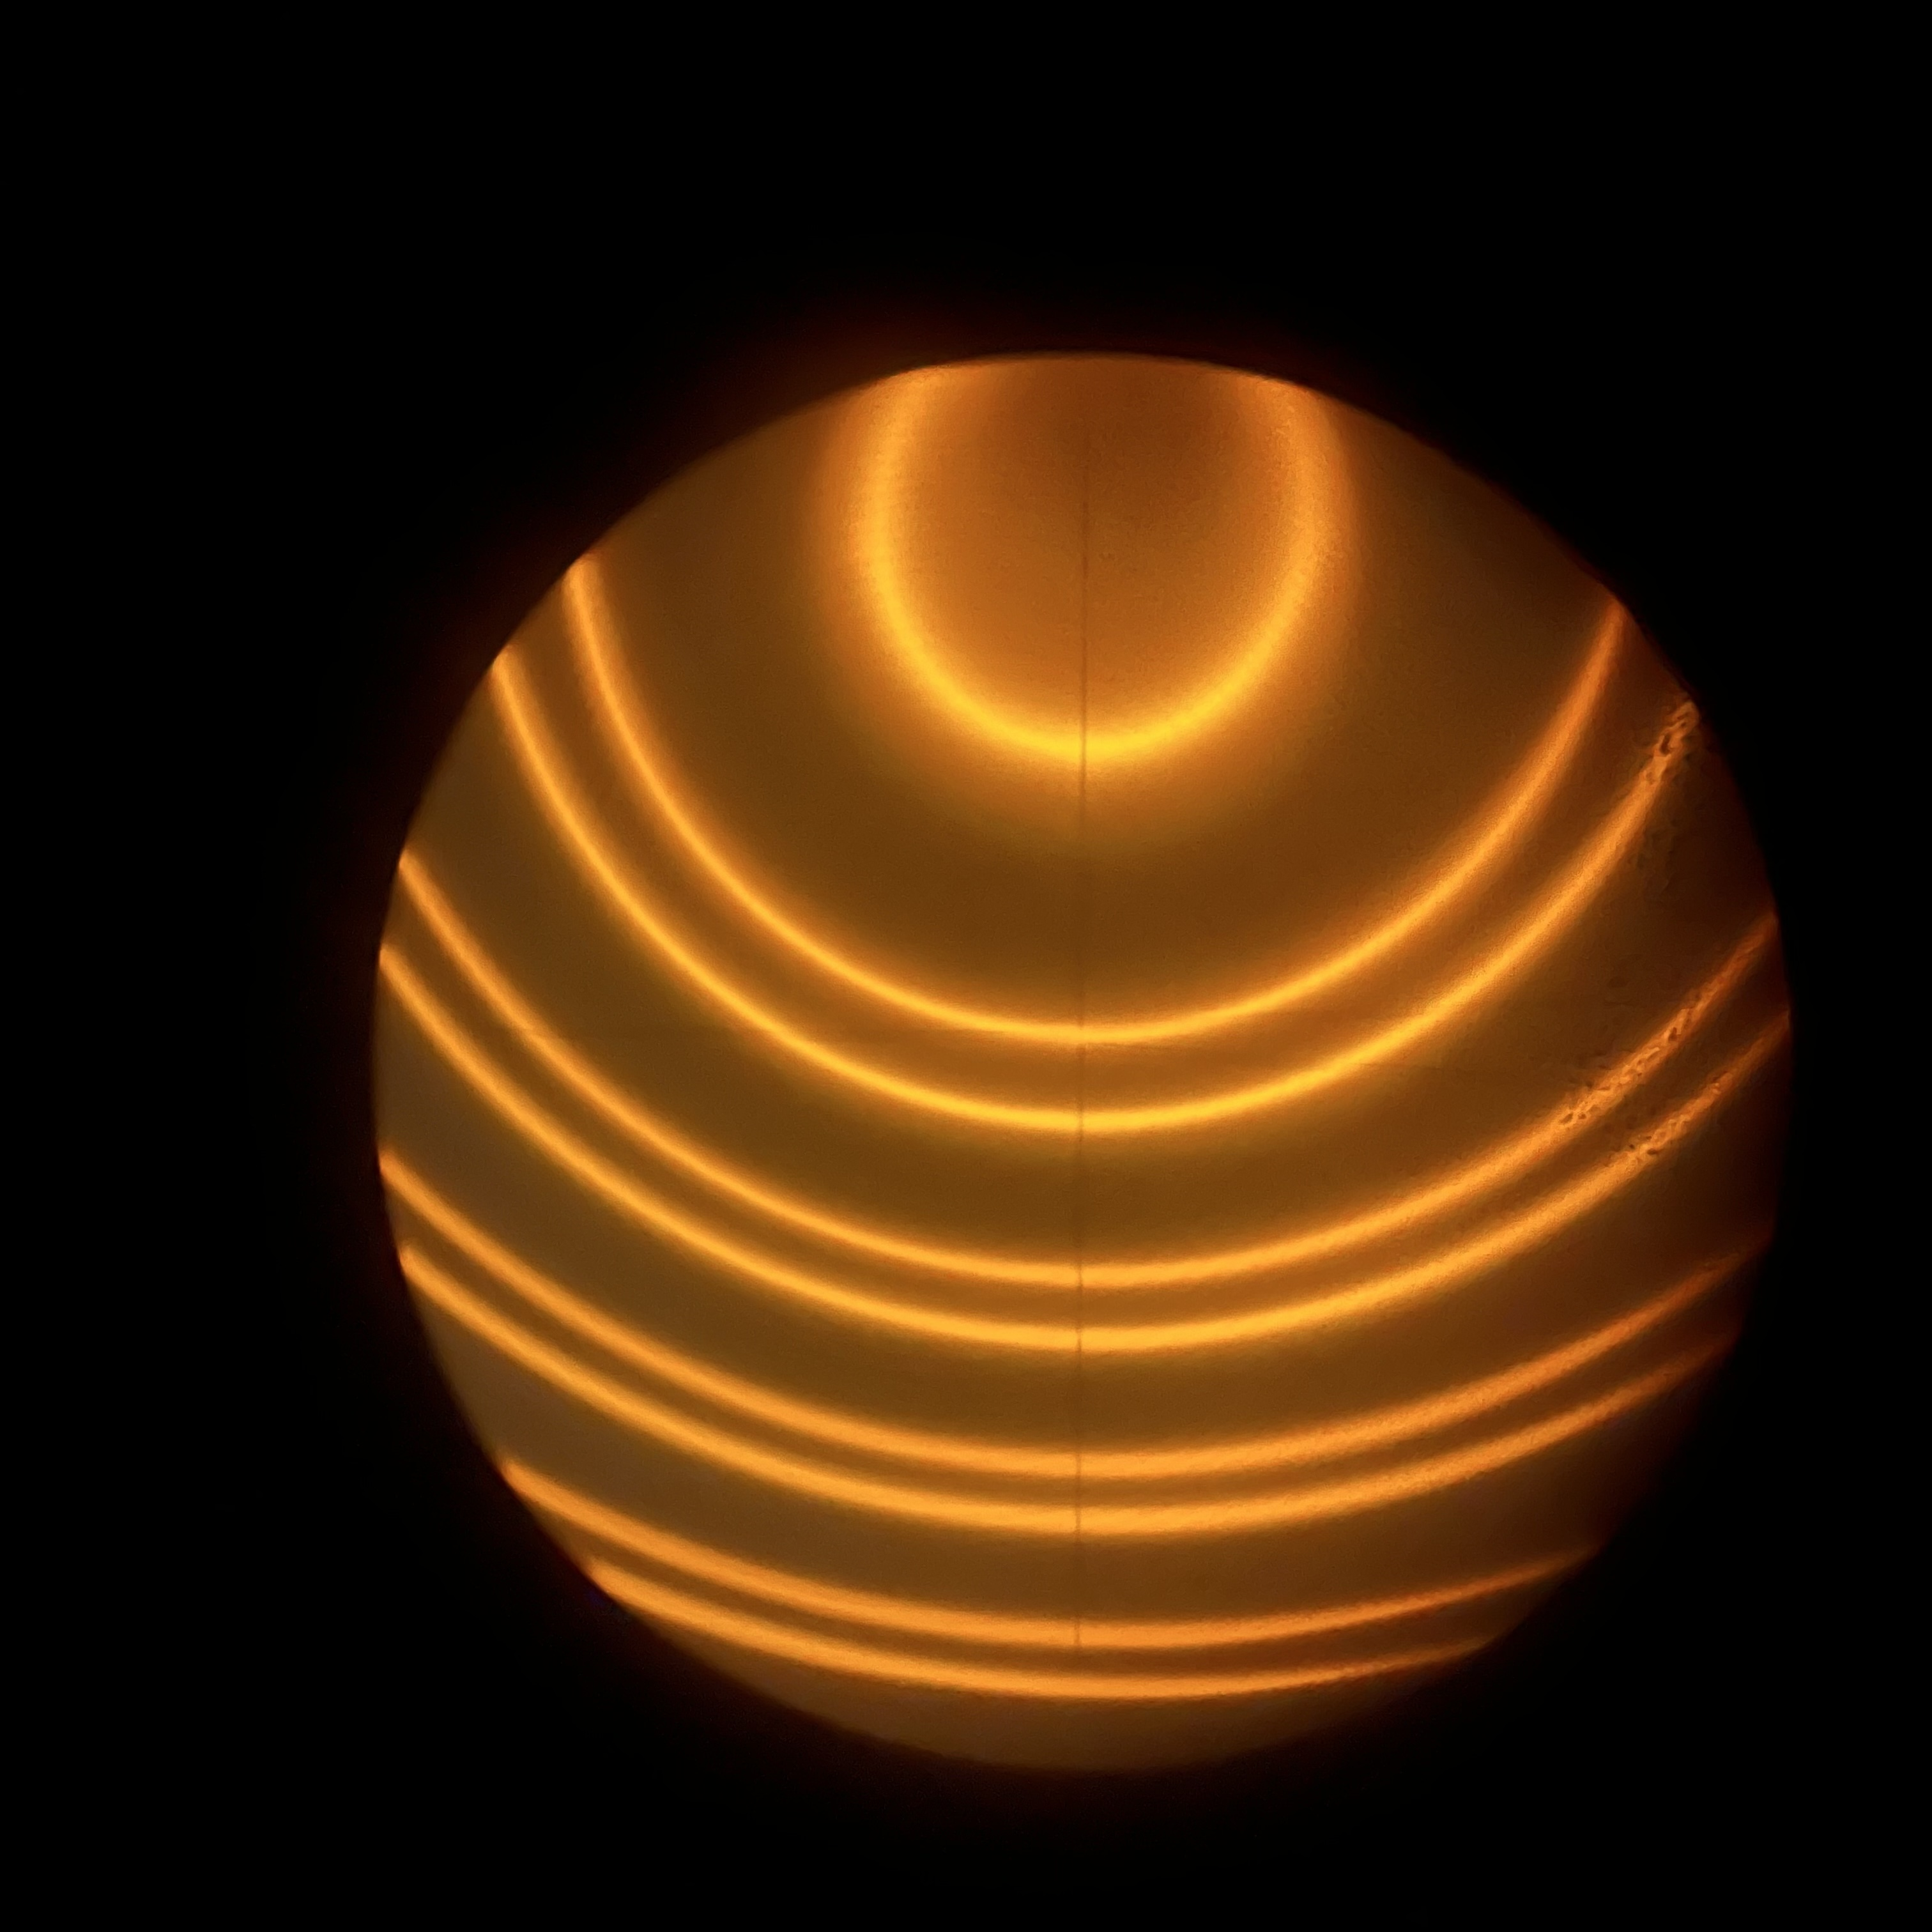
\includegraphics[width=0.95\linewidth]{natr1.png}}
	\end{minipage}
	\begin{minipage}[h]{0.47\linewidth}
		\center{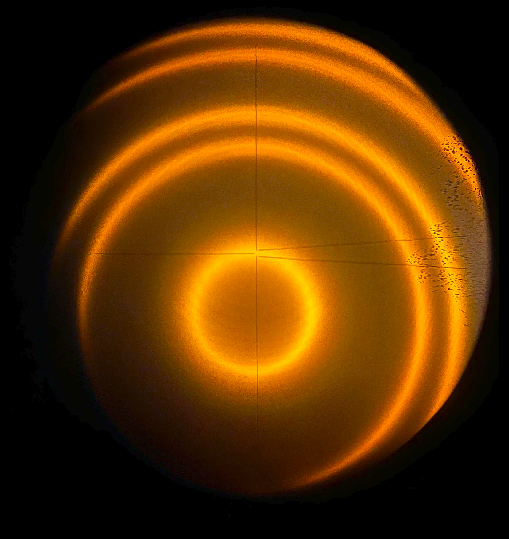
\includegraphics[width=0.95\linewidth]{natr2.png}}
	\end{minipage}
\end{figure}

\begin{table}[!htb]
  \centering
  \caption{Диаметры натриевых колец}
  \begin{tabular}[tb]{|c|c|c|c|c|c|c|c|} \hline
  \textnumero & 
      $R^{\text{up}}_{1}$ мм & 
              $R^{\text{dn}}_{1}$ мм & 
                        $R^{\text{up}}_{2}$ мм & 
                                $R^{\text{dn}}_{2}$ мм &
                                          $D_{1}$ мм &
                                                $D_{2}$ мм &
                                                        $D_{avg}$ мм \\ \hline
  1 & 160.88 & 147.86 & 162.15 & 146.73 & 13.02 & 15.42 & 14.22 \\ \hline
  2 & 164.45 & 144.58 & 165.22 & 143.78 & 19.87 & 21.44 & 20.66 \\ \hline
  3 & 166.88 & 142.13 & 167.58 & 141.44 & 24.75 & 26.14 & 25.45 \\ \hline
  4 & 168.94 & 140.08 & 169.58 & 139.45 & 28.86 & 30.13 & 29.50 \\ \hline
  5 & 170.81 & 138.27 & 171.39 & 137.74 & 32.54 & 33.65 & 33.10 \\ \hline
  6 & 172.54 & 136.63 & 173.00 & 136.07 & 35.91 & 36.93 & 36.42 \\ \hline
  \end{tabular} 
\end{table}

\begin{figure}[htbp]
\centerline{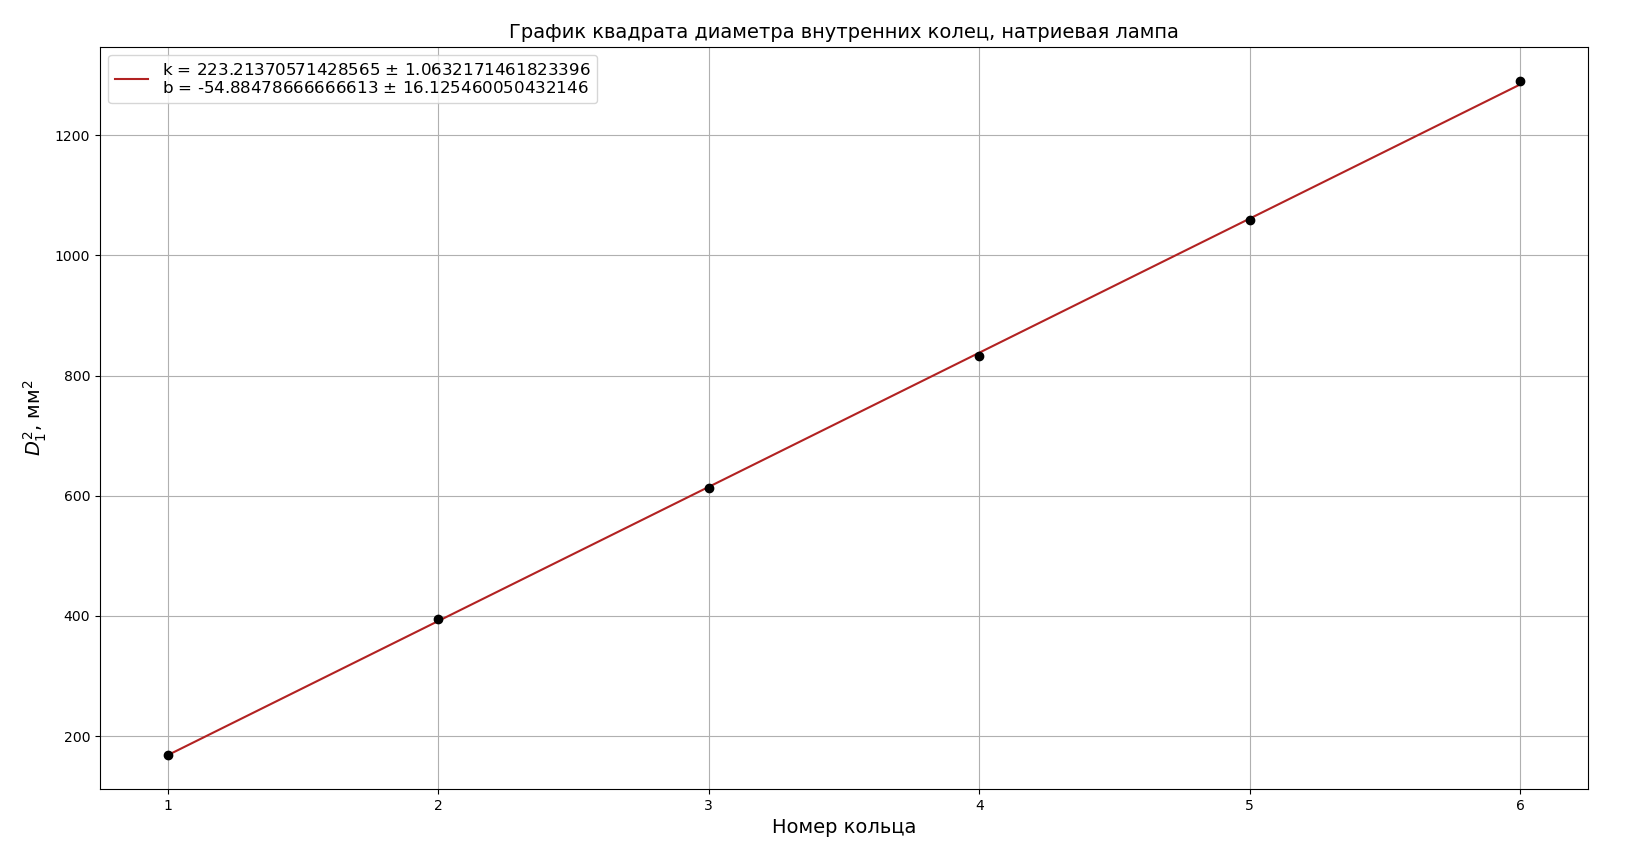
\includegraphics[width=0.99\textwidth]{natgr1.png}}
\end{figure}

\begin{figure}[htbp]
  \centerline{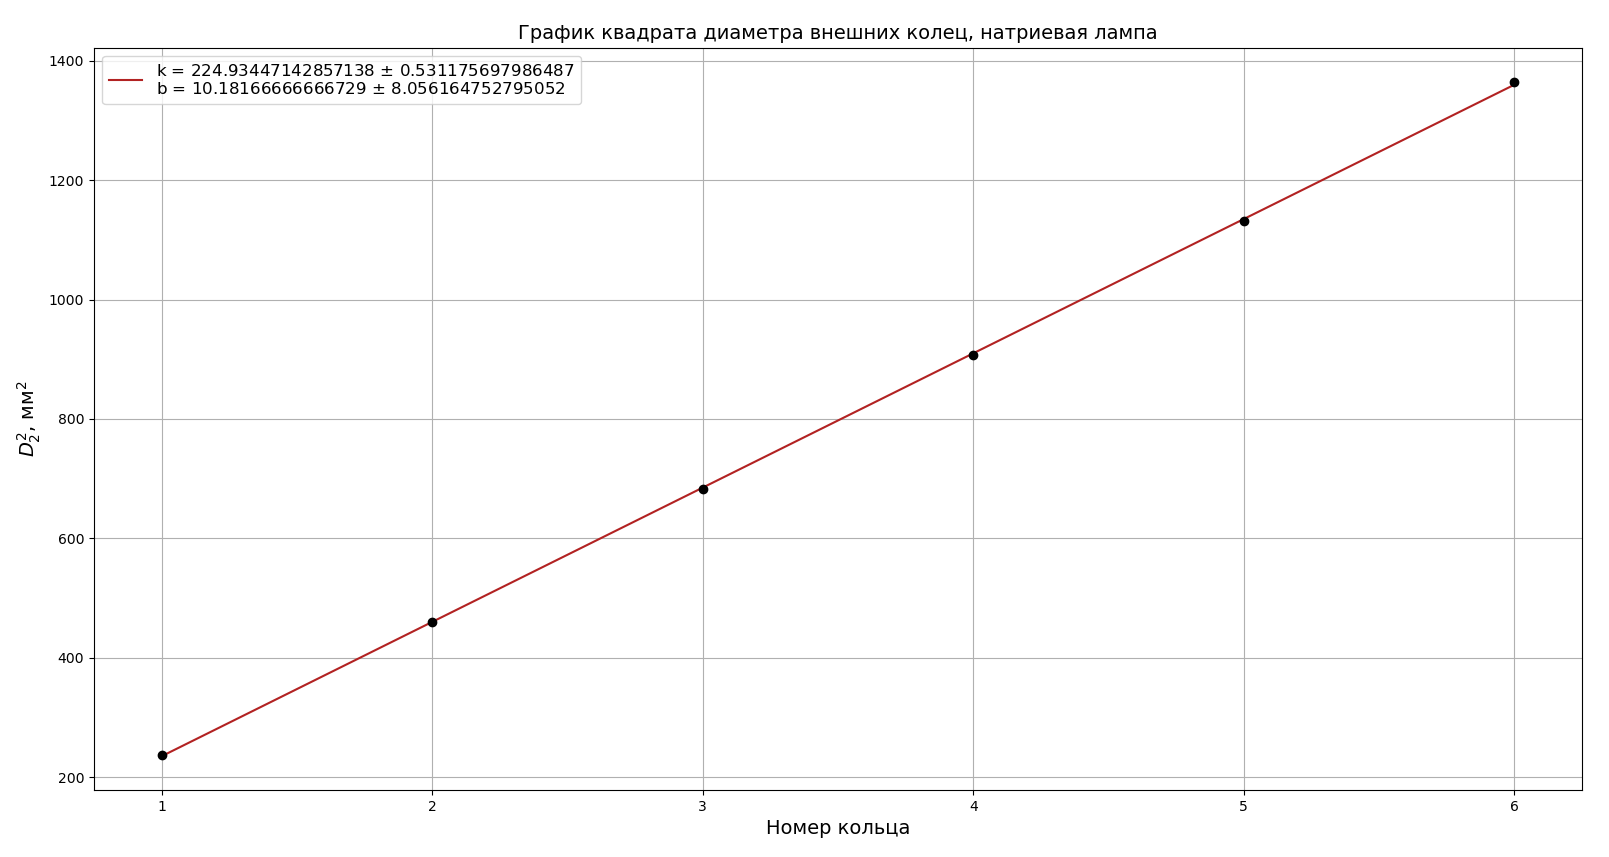
\includegraphics[width=0.99\textwidth]{natgr2.png}}
  \end{figure}

Построим зависимости $D_{n}^{2}$ от $n$. По коэффициентам наклона определим базу интерферометра.
\begin{align*}
  &k_1 = (223.2 \pm 1.1)\ \text{мм}^{2} \\
  &k_2 = (224.9 \pm 0.5)\ \text{мм}^{2} 
\end{align*}
Фокусное расстояние линзы $f = 94$ мм. $\lambda_{Na} = 5893 \text{\AA}$. Отсюда базы интерферометров для 1-ой и 2-ой рыжей линии:
\begin{align*}
    L_1 = (93 \pm 8) \ \text{мкм}
\end{align*}
\begin{align*}
    L_2 = (93 \pm 6) \ \text{мкм}
\end{align*}
Отсюда получаем (погрешность считаем как погрешность среднего плюс систематическая): 
\begin{align*}
L = (93 \pm 10) \ \text{мкм}
\end{align*}

Построим график ${D_{avg}} = F(1/\Delta D)$ для дублета Na. 
\begin{figure}[htbp]
  \centerline{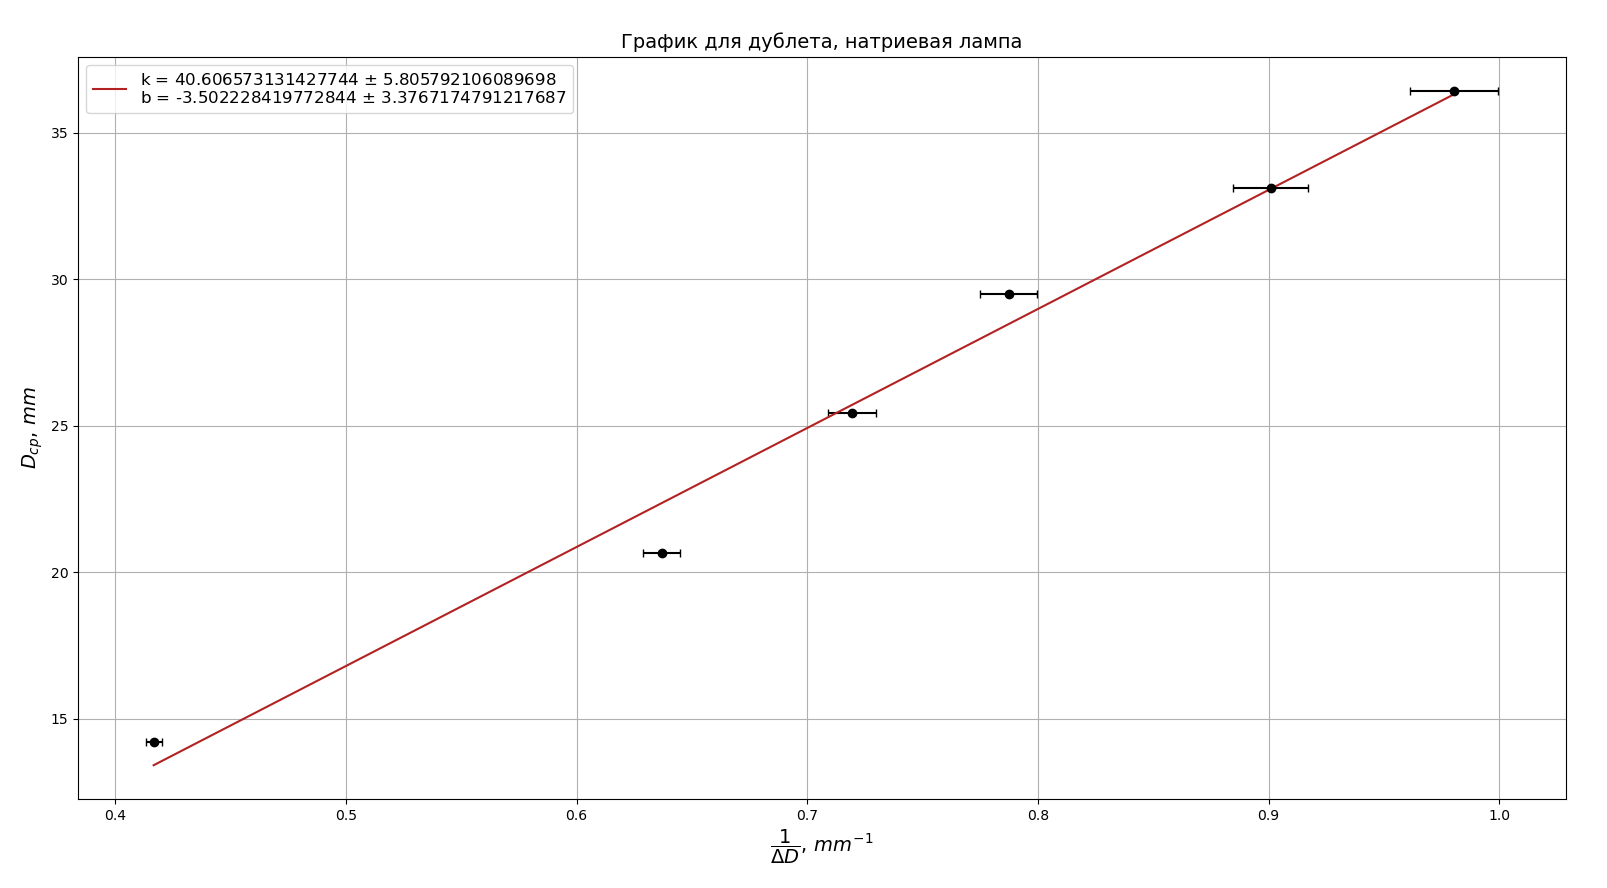
\includegraphics[width=0.99\textwidth]{natgr3.png}}
\end{figure}

Итак, из МНК находим, что
\begin{align*}
    k_3 = \frac{4f^2 \Delta \lambda}{\lambda} = (41 \pm 5)\ \text{мм}^{2}
\end{align*}

\par По формуле из теоретического введения рассчитаем $\Delta \lambda$:
\begin{align*}
    \Delta \lambda_{Na} = (6 \pm 1) \text{\AA}
\end{align*}

\newpage 


\subsection{Ртутная лампа}
Повторим измерения для ртутной лампы. Наблюдаем 17 жёлтых и зелёных колец $\Delta {R} = 0.02$ мм.
\begin{figure}[H]
	\begin{minipage}[h]{0.5\linewidth}
		\center{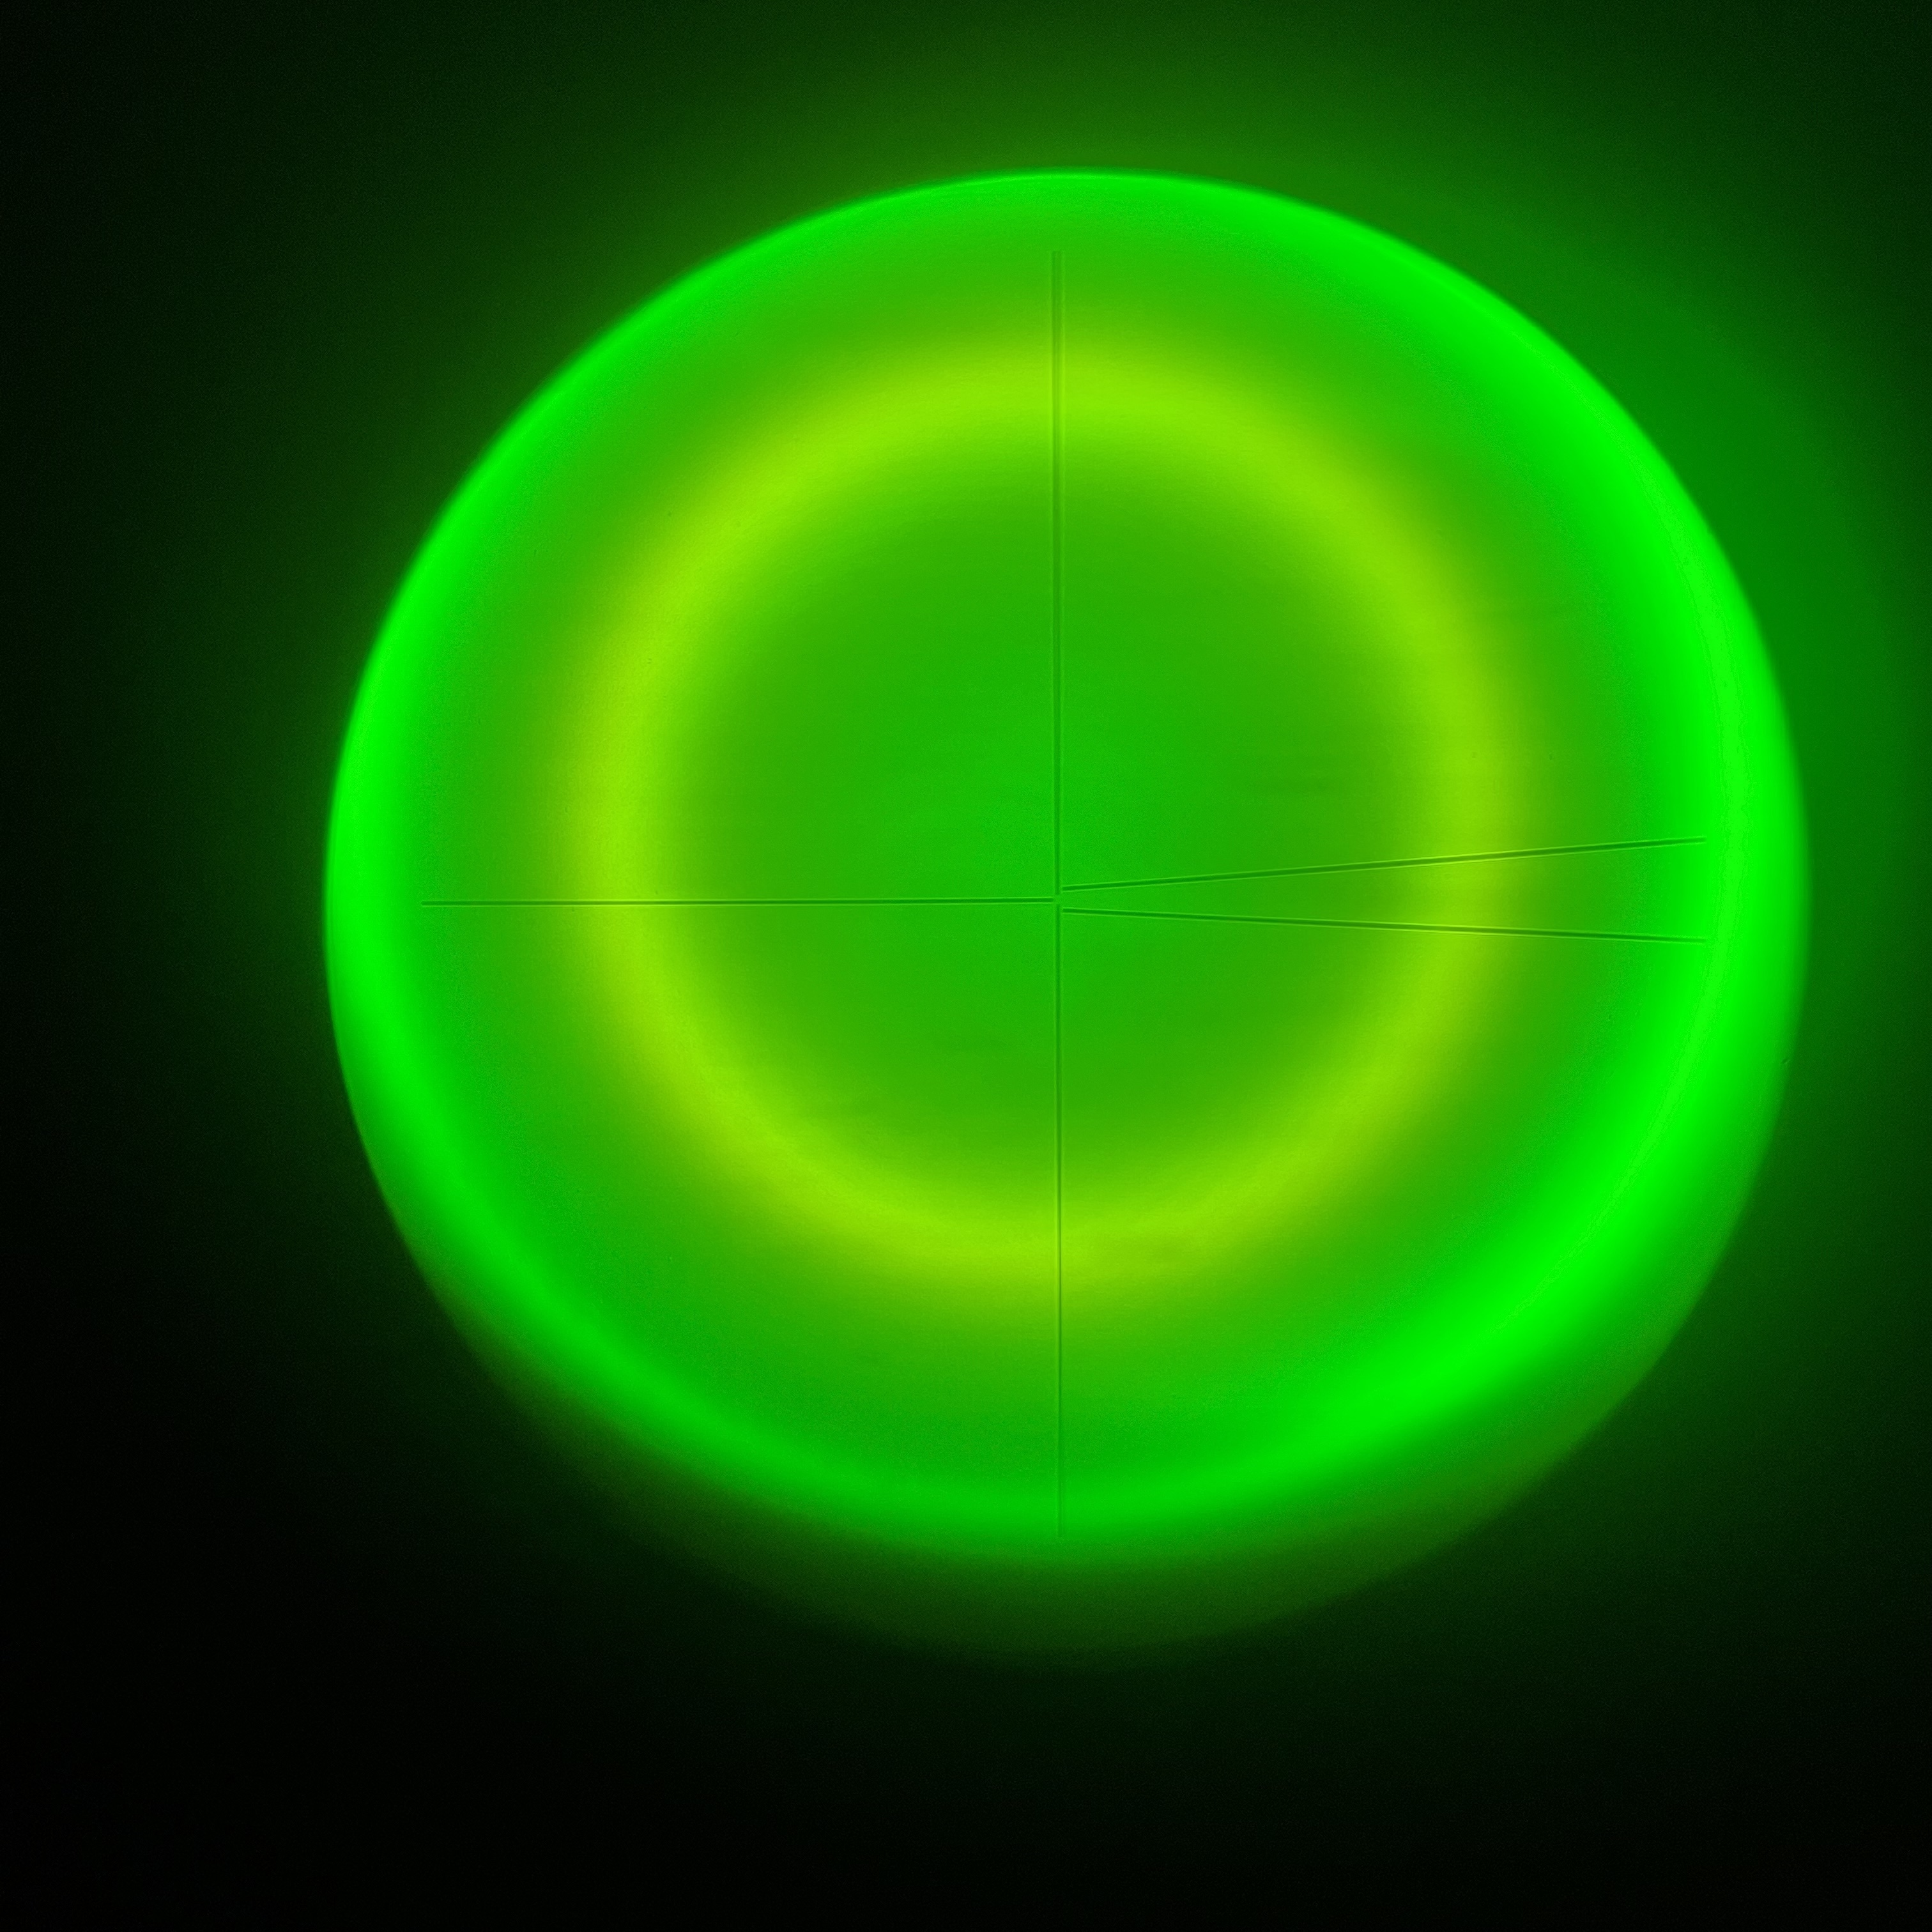
\includegraphics[width=0.95\linewidth]{rtut1.png}}
	\end{minipage}
	\begin{minipage}[h]{0.5\linewidth}
		\center{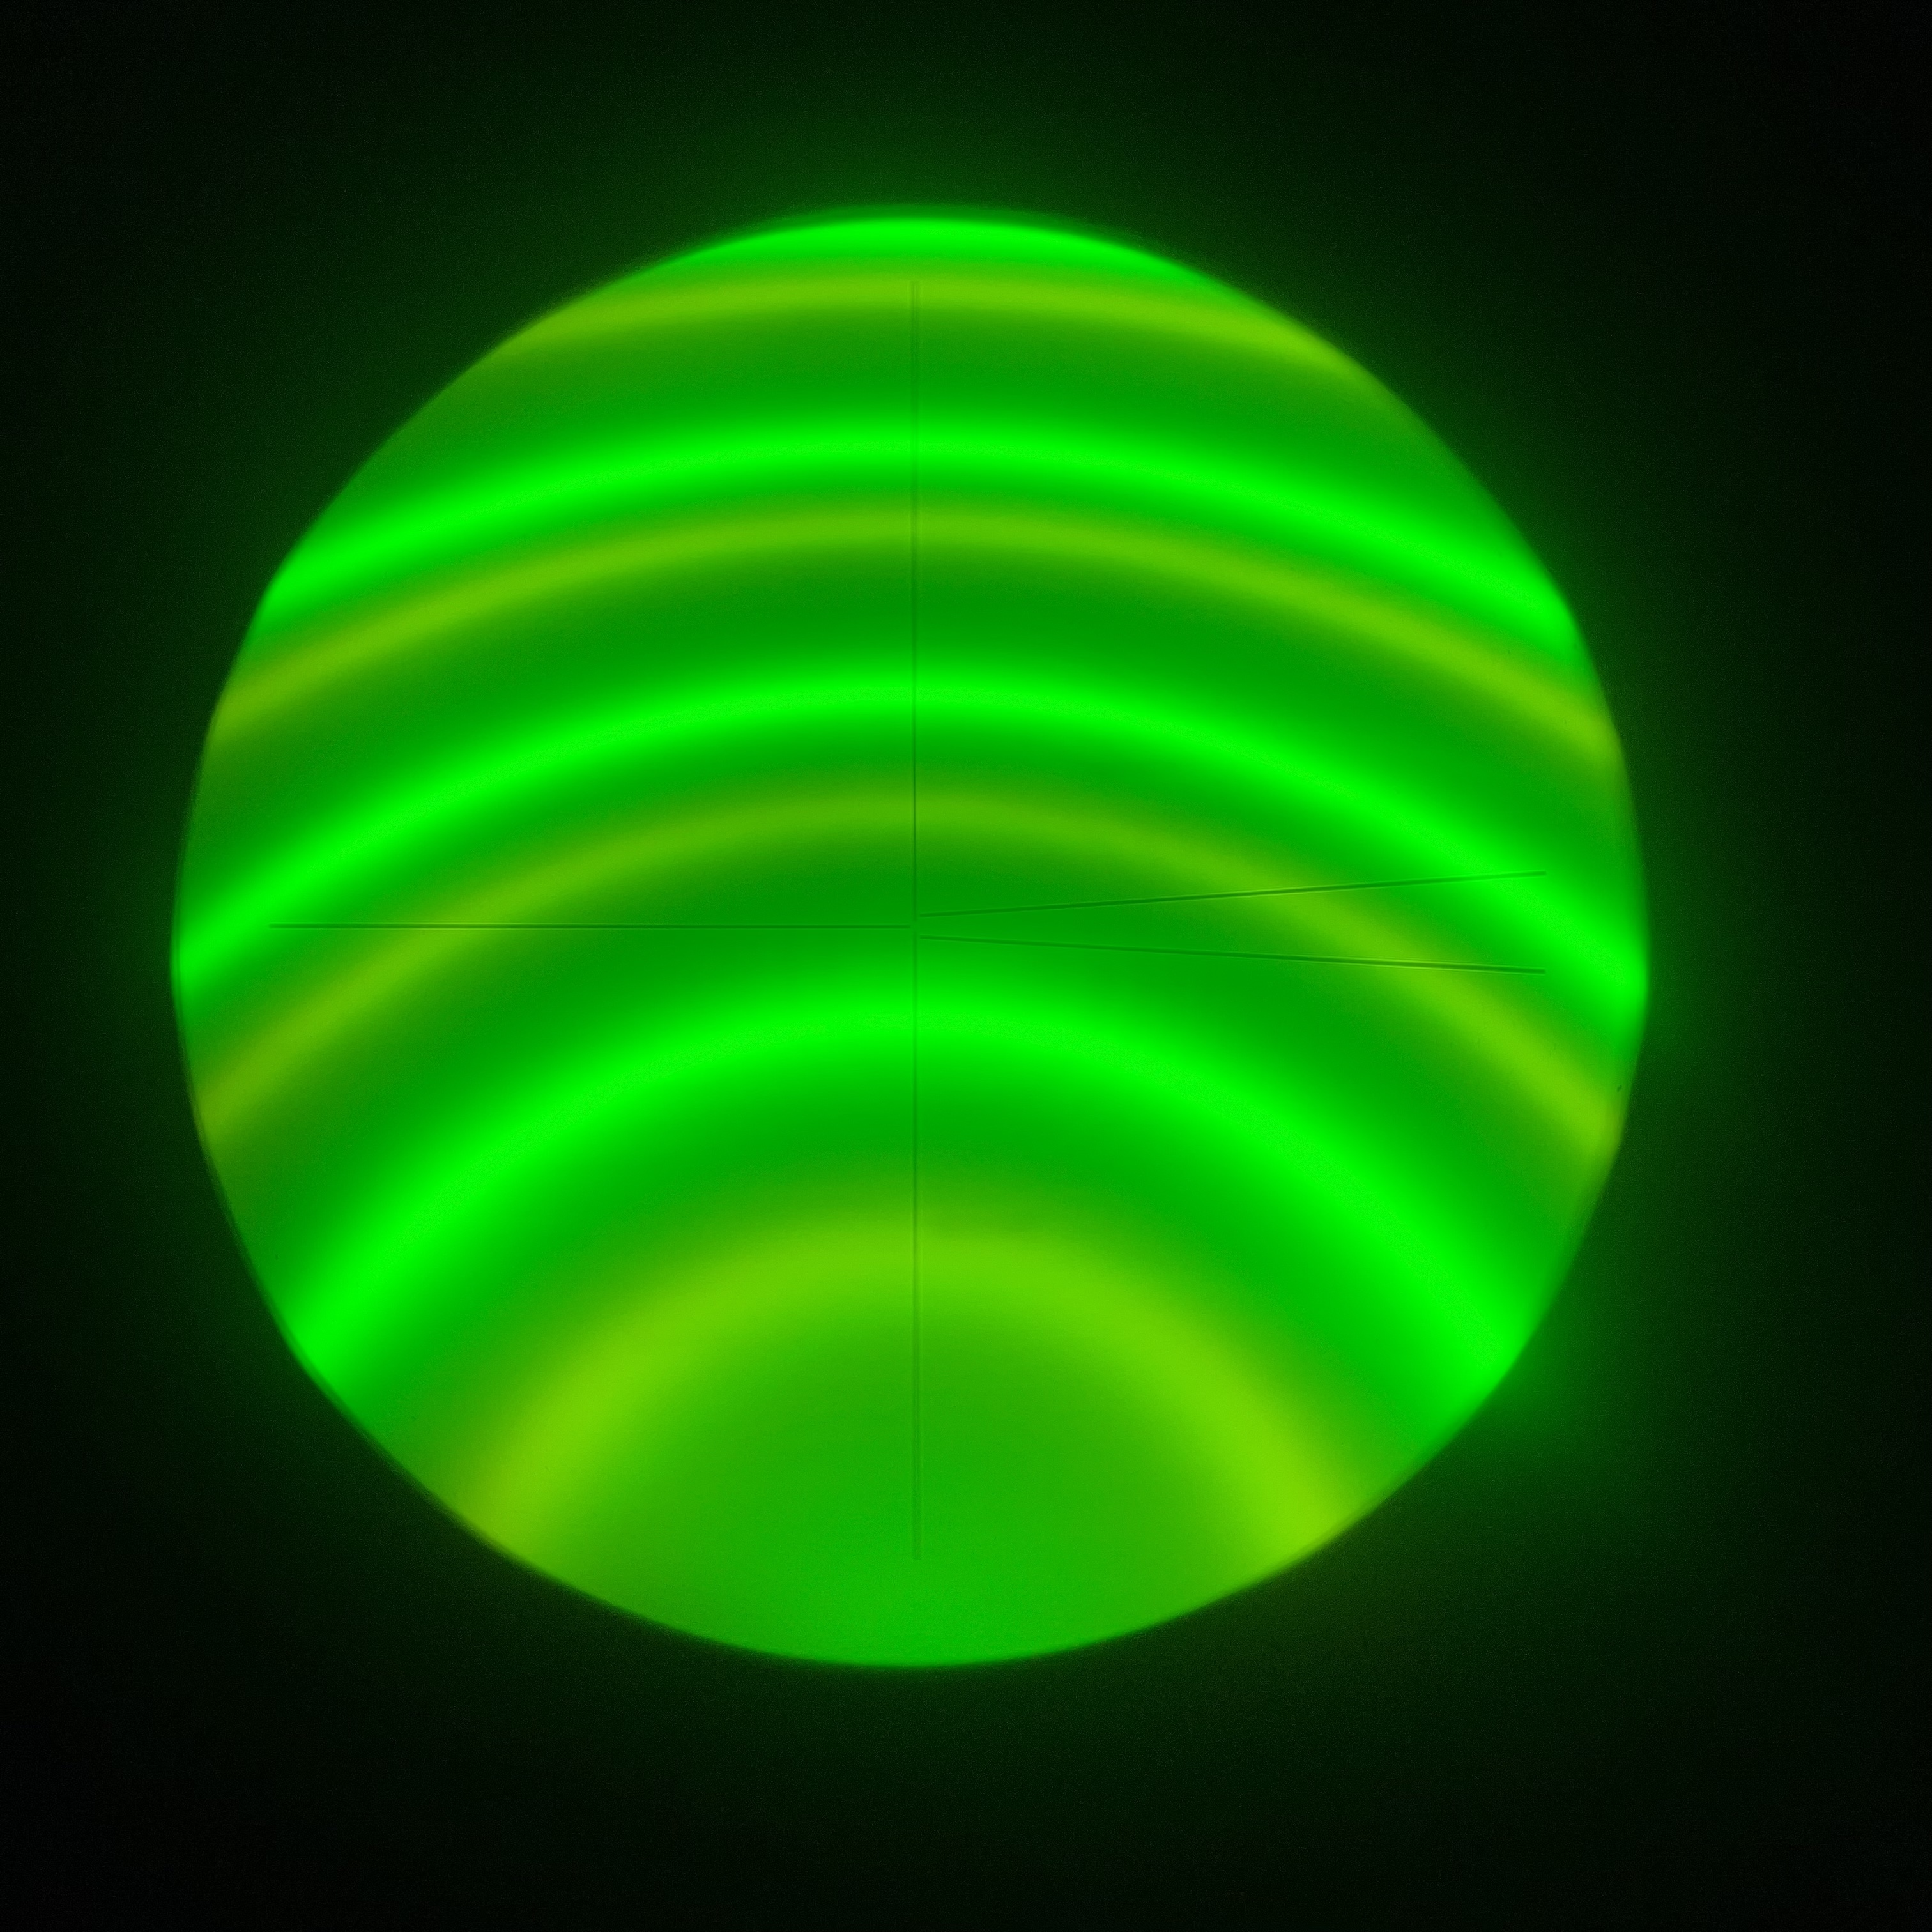
\includegraphics[width=0.95\linewidth]{rtut2.png}}
	\end{minipage}
\end{figure}

\begin{table}[!htb]
  \centering
  \caption{Диаметры ртутных колец}
  \begin{tabular}[tb]{|c|c|c|c|c|c|c|c|} \hline
  \textnumero & 
      $R^{up}_{ylw}$ мм & 
              $R^{dn}_{ylw}$ мм & 
                        $R^{up}_{grn}$ мм & 
                                $R^{dn}_{grn}$ мм &
                                          $D_{ylw}$ мм &
                                                $D_{grn}$ мм \\ \hline
  1 & 177.10 & 169.65 & 179.06 & 167.49 &  7.45 & 11.58 \\ \hline
  2 & 180.83 & 165.70 & 181.90 & 164.62 & 15.13 & 17.29 \\ \hline
  3 & 183.26 & 163.26 & 183.93 & 162.55 & 20.00 & 21.39 \\ \hline
  4 & 185.15 & 161.31 & 185.62 & 160.83 & 23.84 & 24.79 \\ \hline
  5 & 186.74 & 159.70 & 187.04 & 159.33 & 27.04 & 27.71 \\ \hline
  6 & 188.17 & 158.25 & 188.44 & 157.98 & 29.92 & 30.46 \\ \hline
  \end{tabular} 
\end{table}

\begin{figure}[htbp]
\centerline{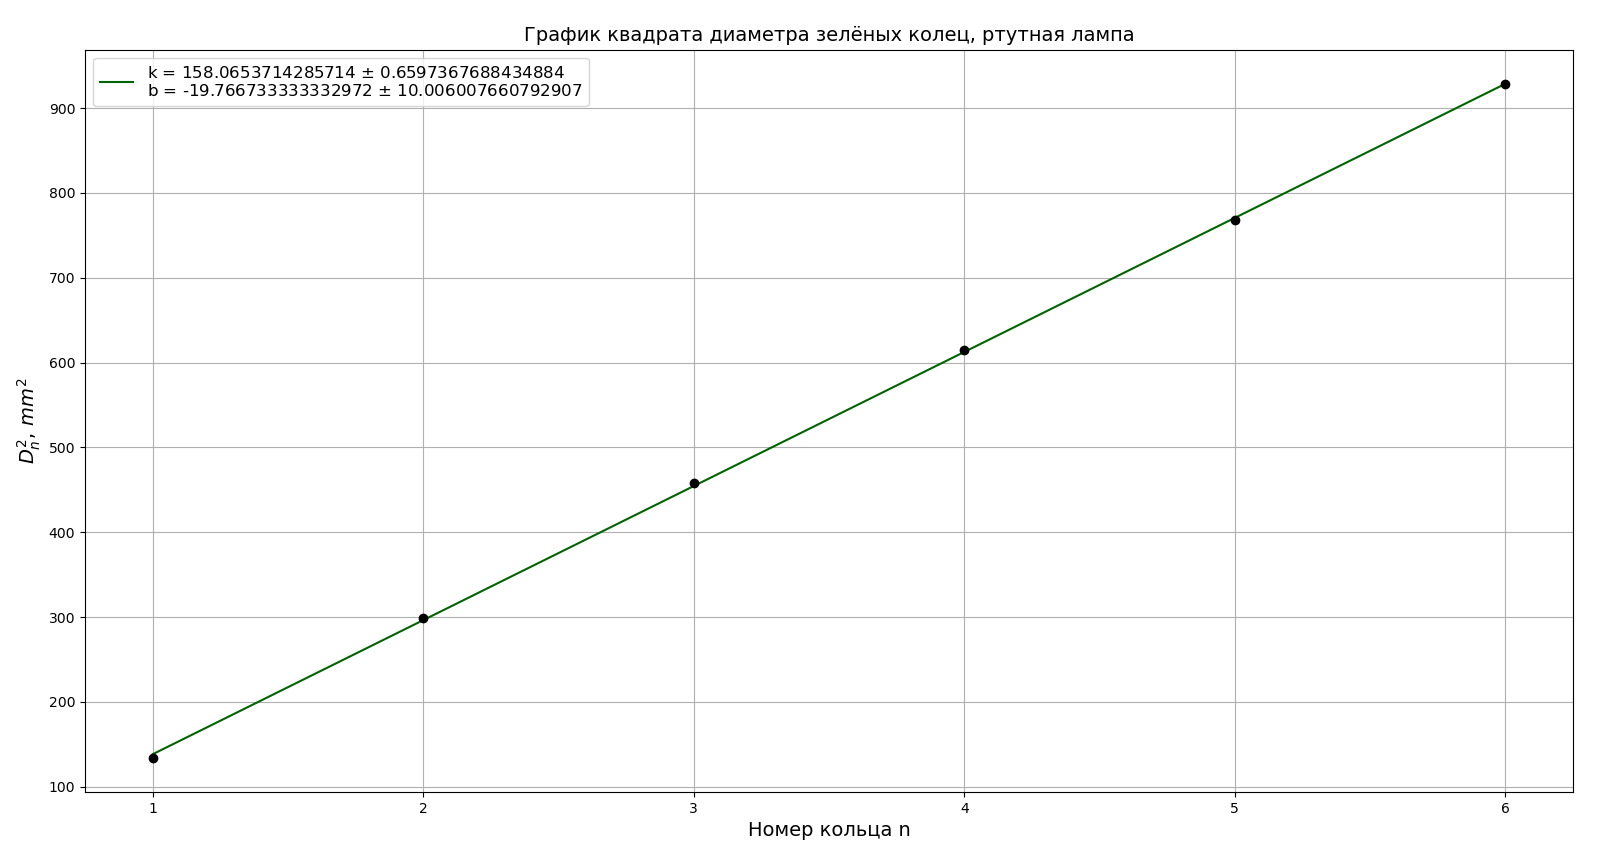
\includegraphics[width=0.99\textwidth]{hggr1.png}}
\end{figure}
\begin{figure}[htbp]
  \centerline{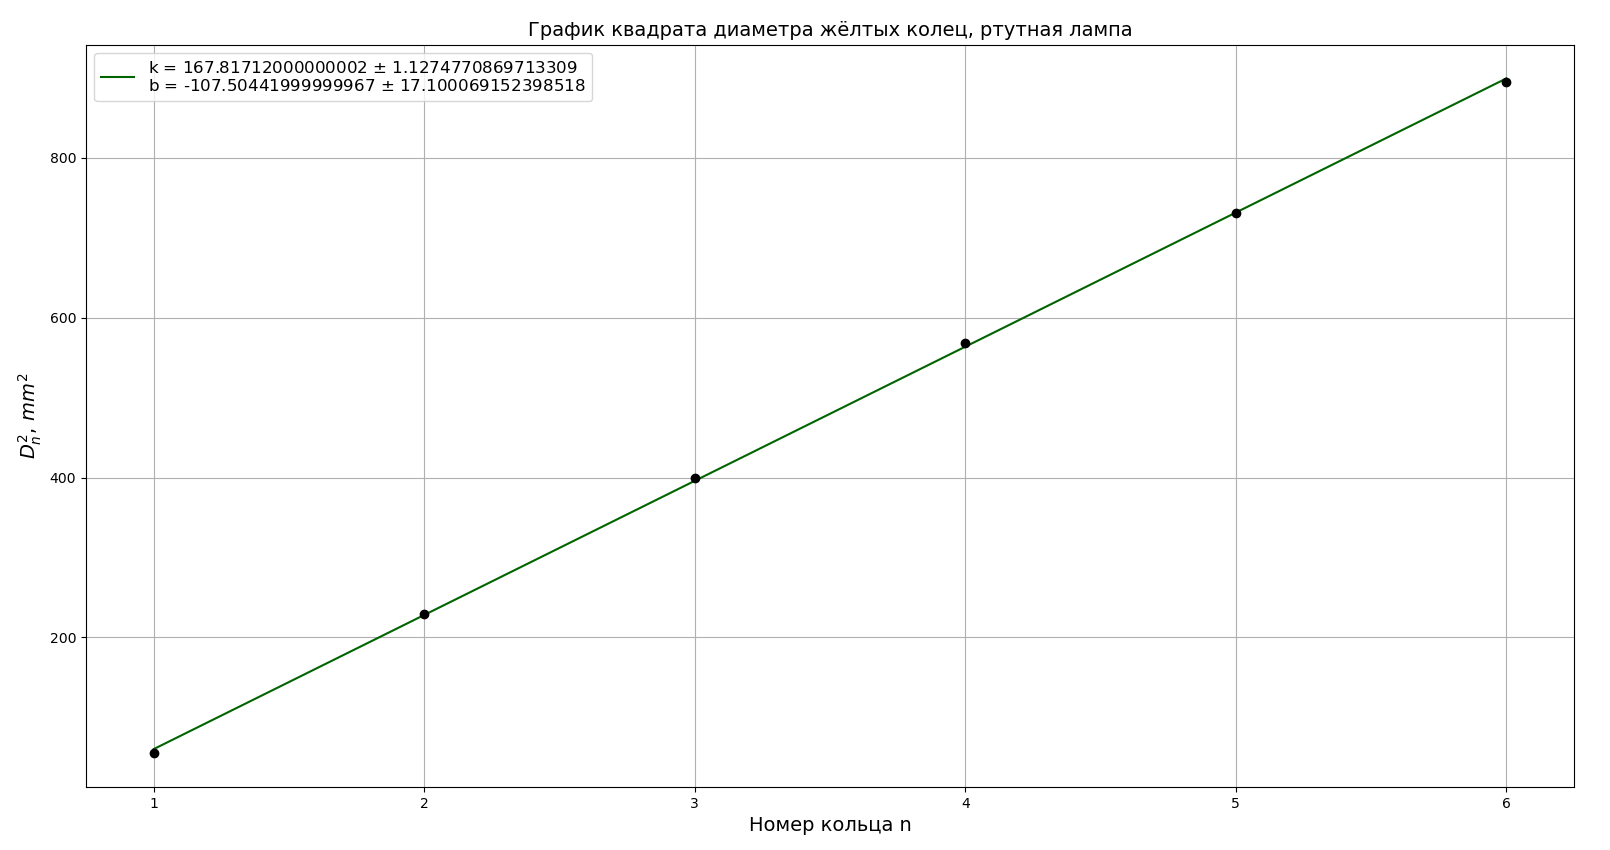
\includegraphics[width=0.99\textwidth]{hggr2.png}}
\end{figure}

\newpage
Построим график зависимости квадрата диаметра колец от номера кольца для обеих линий.
\begin{align*}
  &k_{grn} = (158.1 \pm 0.7)\ \text{мм}^{2} \\
  &k_{ylw} = (167.8 \pm 1.1)\ \text{мм}^{2}
\end{align*}
Вычислим базу $L$ интерферометра по формуле из теоретических сведений. $\lambda(Hg)_{grn} = 5461 \text{\AA}$. $\lambda(Hg)_{yel} = 5780 \text{\AA}$. $f = 50$ мм. Погрешность здесь вычисляем с помощью формулы для погрешности косвенных измерений
через частные производные:
\begin{align*}
   \frac{\lambda}{L} = \frac{1}{4f^2}\frac{\Delta(d^2_i)}{\Delta(i)},
\end{align*}
Итого: 
\begin{align*}
    L_{grn} = (34.5 \pm 0.2) \ \text{мкм} \\
    L_{ylw} = (34.4 \pm 0.3) \ \text{мкм}
\end{align*}
Отсюда получаем:
\begin{align*}
  L = (34.5 \pm 0.5) \ \text{мкм}
\end{align*}

Для ртутной лампы желтого дуплета не обнаружено. Попытка взять отдалённые друг от друга жёлтые кольца не увенчалась успехом (график явно нелинейный). 
Аналогично с парами жёлтых и зелёных колец. В связи с этим $\Delta \lambda_{Hg}$ посчитать не можем.
%будем считатать по формуле:
% \begin{equation}
%   \Delta \lambda_{Hg} = \frac{\lambda^{2}}{2L} = (4.8 \pm 0.3) \text{\AA}
% \end{equation}

\subsection{Линейная дисперсия}
Для нахождения линейной дисперсии воспользуемся следующей формулой.
\begin{equation}
    D_{exp} = \frac{\Delta D}{2 \Delta \lambda} \text{ мм/}{\text{\AA}}
\end{equation}
Подставляя туда $\Delta D$ для пары колец максимального диаметра, будем сравнивать результат с теоретическим значением, даваемым формулой
\begin{equation}
    D_{thr} = \frac{2f^2}{\lambda D}.
\end{equation}

Для натрия получаем:

\begin{align*}
    D^{Na}_{exp} = (0.201 \pm 0.006)\, \text{мм/}{\text{\AA}}, \quad D^{Na}_\text{thr} = 0.198\, \text{мм/}{\text{\AA}} \\
\end{align*}
--- как видим, полученное экспериментальное значение близко к табличному.

\subsection{Разрешающая способность}
Измерим толщины колец для натриевой и ртутной ламп.
Для натрия толщина первого желтого кольца:
\begin{align*}
\delta r_{Na} = (0.32\pm0.01)\ \text{мм}
\end{align*} 
Из этих данных получим аппаратную разрешающую способность:  
\begin{align*}
  &R_{Na} = \dfrac{\lambda}{\delta \lambda} \approx \dfrac{4f^2}{D \delta r} = 8500 \pm 100 \quad \text{для первой желтой линии}\\
\end{align*}

Для ртутной лампы толщина первого желтого кольца 
\begin{align*}
\delta r_{ylw} = (0.66\pm0.02)\ \text{мм}
\end{align*}
зеленого: 
\begin{align*}
\delta r_{grn} = (0.30\pm0.02)\ \text{мм}
\end{align*}
Из этих данных получим аппаратную разрешающую способность:  
\begin{align*}
  &R_{\text{апп}} = \dfrac{\lambda}{\delta \lambda} \approx \dfrac{4f^2}{D \delta r} = 2000 \pm 100 \quad \text{для желтой линии}\\
  &R_{\text{апп}} = \dfrac{\lambda}{\delta \lambda} \approx \dfrac{4f^2}{D \delta r} = 2900 \pm 100 \quad \text{для зеленой линии}
\end{align*}
Откуда среднее значение
\begin{align*}
R_{Hg} = 2500 \pm 200
\end{align*}

\subsection{Прочие характеристики интерферометра}
Оценим максимальный порядок интерференции $m$ для желтых линий натрия и ртути:

$$ m_\text{Na} = \frac{2L \cos \theta}{\lambda} \approx \frac{2L}{\lambda} = 305 \qquad \qquad m_\text{Hg} \approx \frac{2L}{\lambda} = 119$$

Кроме того, оценим дисперсионную область:

$$ \Delta \lambda_{Na} = \frac{\lambda^2}{2 L}= 19 \; \text{\AA}  \qquad \qquad  \Delta \lambda_{Hg} = \frac{\lambda^2}{2 L}= 48 \; \text{\AA}$$

Найдём добротность:
$$ Q_{Na} = \frac{2 \pi L}{\lambda (1 - r)} = 6400 \pm 500 \qquad \qquad Q_{Hg} = \frac{2 \pi L}{\lambda (1 - r)} = 2500 \pm 50 $$
при $ r = 0.85 $

Отсюда получаем число интерферирующих лучей: 
$$ N_{Na} = \frac{Q}{m} = 21 \qquad \qquad N_{Hg} = \frac{Q}{m} = 21 $$


\section{Вывод}
В работе были измерены спектральные характеристики интерферометра Фабри-Перо в случае наблюдения натриевой и ртутной лампы. 

Была определена линейная дисперсия $D$ интерферометра. Полученное значение близко к теоретическому

Была определена дисперсионная область интерферометра $\Delta \lambda$ -- получившиеся довольно малые значения согласуются с действительностью
(интерферометр Фабри-Перо обладает очень большой аппаратной разрешающей способностью, но используется только для анализа довольно узких спектров).

Была определена аппаратная разрешающая способность $R_{\text{апп}}$ интерферометра. Полученные значения $\sim 10^{4}$ по порядку величины согласуются с реальными значениями
этой характеристики для интерферометра Фабри-Перо.

Также в результате работы была измерено число интерферирующих лучей -- полученное значение для натриевой лампы довольно неплохо совпадает с
теоретическим значением. К сожалению, часть вычислений для ртутной лампы проведена не была, так как отсутствовал жёлтый дуплет.
\end{document}